\documentclass[11pt]{article}
\usepackage{euscript}

\usepackage{amsmath}
\usepackage{amsthm}
\usepackage{amssymb}
\usepackage{epsfig}
\usepackage{xspace}
\usepackage{color}
\usepackage{url}
\usepackage{subfig}
\usepackage{float}
\usepackage{array}
\graphicspath{ {images/} }
%%%%%%%  For drawing trees  %%%%%%%%%
\usepackage{tikz}
\usetikzlibrary{calc, shapes, backgrounds}

%%%%%%%%%%%%%%%%%%%%%%%%%%%%%%%%%
\setlength{\textheight}{9in}
\setlength{\topmargin}{-0.600in}
\setlength{\headheight}{0.2in}
\setlength{\headsep}{0.250in}
\setlength{\footskip}{0.5in}
\flushbottom
\setlength{\textwidth}{6.5in}
\setlength{\oddsidemargin}{0in}
\setlength{\evensidemargin}{0in}
\setlength{\columnsep}{2pc}
\setlength{\parindent}{1em}
%%%%%%%%%%%%%%%%%%%%%%%%%%%%%%%%%


\newcommand{\eps}{\varepsilon}

\renewcommand{\c}[1]{\ensuremath{\EuScript{#1}}}
\renewcommand{\b}[1]{\ensuremath{\mathbb{#1}}}
\newcommand{\s}[1]{\textsf{#1}}
\newcommand{\tb}[1]{\textbf{#1}}

\newcommand{\E}{\textbf{\textsf{E}}}
\renewcommand{\Pr}{\textbf{\textsf{Pr}}}
\newcommand*{\escape}[1]{\texttt{\textbackslash#1}}


\title{\textbf{\underline{Asmt 5: Regression}}}
%\footnote{\s{CS 6140  Data Mining; \;\; Spring 2015 \hfill
%Instructor: Jeff M. Phillips, University of Utah}
%}

\author{Anirudh Narasimhamurthy(u0941400)}

\begin{document}
\maketitle

\section{Singular Value Decomposition}

\begin{itemize}
	
	
	\item[] In this part of the assignment we will experiment with Singylar Value Decomposition(SVD) technique by applying it on our given matrix A
	
	\item[] \underline{\textbf{1.A.}}
	
	 \textbf{$L_2$ norm of the difference between A and Ak:}\\	
	 
	The $L_2$ norm was computed for the difference between A and Ak for each value of k from k=1 to 10, using the expression \textbf{norm(A-Ak,2)}. The values are tabulated below:
	
	\begin{table}[h]
		\centering
		\begin{tabular}{|c|c|}
			\hline
			\textbf{k}  & \textbf{norm(A-Ak,2)}\\
			\hline
			1 &  20.2937  \\
			\hline
			2 &  15.1907 \\
			\hline
			3 &  11.5438  \\
			\hline
			4 &  7.5638  \\
			\hline
			5 &  5.9804  \\
			\hline
			6 &  5.2966  \\
			\hline
			7 &  4.0402  \\
			\hline
			8 &  3.6567  \\
			\hline
			9 &  1.6420  \\
			\hline
		    10 &  1.4102  \\
		    \hline	
		\end{tabular}
		\caption{$L_2$ norm difference between A and Ak for k=1 to k=10 }
		\label{t2}
	\end{table}
	
	\item[] \underline{\textbf{1.B.}}
	
	The smallest value of k so that $L_2$ norm of A-Ak is less than 10\% of that of A is $\boxed{\textbf{k=7}}$.
	
	I had a check condition inside my MATLAB code to print the k value when 10\% of A was greater than $L_2$ norm of A-Ak. 
	
	10\% of A gave a value of \textbf{4.1584}. From the table in 1.A we see that the $L_2$ norm of A-Ak for k=6 is 5.2966 and for k=7 it is 4.0402 which is less than 10\% of the value of A
	
	\item[] \underline{\textbf{1.C.}}
	
	We are asked to treat the matrix as 1125 points in 30 dimensions and are asked to plot the points in 2-dimensions in the way that minimizes the sum of the residuals squared.\\
	
	We know  $A= USV^T$ and in our case the number of dimensions was 30. If we want it in 2 dimensions or k dimensions, then it would effectively be $Ak*V= UkSkV^T V$. V being a square matrix the product of V. $V^T$ would be 1.
	\\
	
	This is equivalent to plotting \textbf{U2*S2  where U2=U(:,1:2) and S2=S2(1:2,1:2).} This will give us a good approximation of the input from 30 dimensions to 2-dimensions which minimizes the sum of residuals squared as SVD guarantees us this property. The resultant matrix of U2*S2 is a 1125x 2 double matrix. I have used \textbf{scatter()} function in MATLAB to plot the x and y values. 

	\begin{figure}[H]%
		\centering
		\subfloat[ 2-dimensional plot of the points ]{{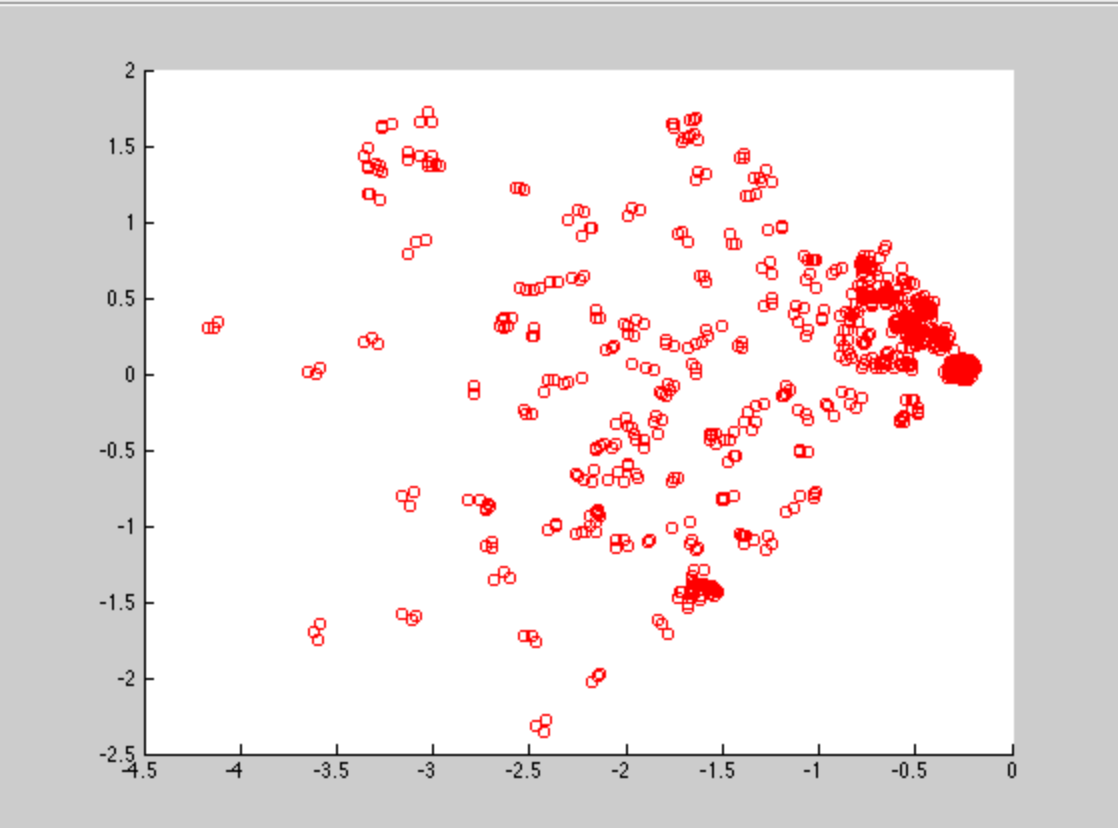
\includegraphics[width=7cm]{plot1c} }}%
	\end{figure}	

The above graph represents the points or the co-ordinates and hence doesn't rquire any labeling of axis. If required, the X-axis would be x co-ordinates of the points and the Y-axis would be the y co-ordinates of the points.
	
\end{itemize}


\section{Frequent Directions}

\begin{itemize}
	\item[] \underline{\textbf{2.A.}}
	
	I completed the function definition in the stub file FD.m\\
	
	The error is measured by :\\
	norm(A' * A - B'*B,2)\\
	
	The Forbenius norm was calculated using the Matlab function \\
	
	 When the matlab code was run, at l=4 the error is 255.2102 which is less than ${||A||}_{F}^{2}/10 =2679.3/10= 267.93$
	This is the clsoest value to the bound.For l=5 it will exceed this.
	Hence the empirical bound of l is$\boxed{ l=4.}$ 
	
	The theoretical bound in this case is given by $l=\frac{1}{\epsilon} $.  $\epsilon$ being 0.1, since we are asked to find the bound of $||A||_F^2/10 $we have $\boxed{l=10}$.
	
	
	
	\item[] \underline{\textbf{2.B.}}
	
	In our problem we have :\\
	\item[] ${||A-A\Pi_{B_k}||}_{F}^{2}    \leq 1.1   \cdot {||A-A_k||}_{F}^{2}$
	
	The theoretical bound is given by:\\
	\item[] 	${||A-A\Pi_{B_k}||}_{F}^{2}    \leq \frac{l}{l-k}   \cdot {||A-A_k||}_{F}^{2}$
		
	Equating the two, we obtain the theoretical bounds as follows:
	
	
	\item[] $\frac{l}{l-k} =1.1$
	\item[] 	$l=1.1(l-k)$
		\item[] $-0.1l=-1.1k$
		\item[] $\boxed{l=11k}$
	
	Substituting the different values of 'k' , the theoretical l values can be obtained. The values from the experiments for l have also been tabulated in the table below:
	
	\begin{table}[h]
		\centering
		\begin{tabular}{|c|c|c|}
			\hline
			\textbf{k}  & \textbf{Theoretical bound l (l=11*k)} & \textbf{Empirical bound}\\
			\hline
			1 &  11 & 2 \\
			\hline
			2&  22 & 3\\
			\hline
			3 &  33  & 4\\
			\hline
			4 &  44  & 6 \\
			\hline
			5 & 55 & 6\\
			\hline
			6 & 66 & 8\\
			\hline
			7 & 77 & 9\\
			\hline	
		\end{tabular}
		\caption{Theoretical bound and Empirical bound for l value for different k values}
		\label{t2}
	\end{table}
	
	
	
	
\end{itemize}


\section{Linear Regression}

\begin{itemize}
	\item[] \underline{\textbf{3.A.}}
	
	\textbf{Error in the estimation of of $\hat Y$}
	
	\item[] In this section we are asked to solve the co-efficients of C using Least Squares and for Cs using Ridge Regression with s=\{0.1, 0.3, 0.5, 1.0, 2.0\}.
	
	\item[] The formula used for computing co-efficients for each of the method is given below:
	
	\textbf{Least Squares: C= inverse(X' * X) *X' * Y} \\
	\textbf{Ridge Regression: Cs= inverse(X' *X + $s^2 $ *eye(12)) * X' *Y} \\
	
	Here X' denotes the transpose of the matrix X.
	
	\item[] After solving and finding the co-efficients, each of which were 12 x 1 vector, the error was estimated using the expression norm(Y- X*C,2). The estimates of error are tabulated below:
	
		\textbf{\underline{Least Squares Error Estimates for input X and Y:}}
		
		Error via least squares= norm(Y- X*C,2)= \textbf{7271.445397}
	
	\pagebreak
	\textbf{\underline{Ridge Regression Error Estimates for different values of s}}
	
	
	\begin{table}[h]
		\centering
		\begin{tabular}{|c|c|}
			\hline
			\textbf{s}  & \textbf{Error Estimate= norm(Y-X*Cs,2)}\\
			\hline
			0.1 &  7271.445397  \\
			\hline
			0.3&  7271.445403 \\
			\hline
			0.5 &  7271.445444  \\
			\hline
			1.0 &  7271.446147  \\
			\hline
			2.0 & 7271.457285 \\
			\hline
			\end{tabular}
		\caption{Error estimates for ridge regression for different values of s for input X and Y }
		\label{t2}
	\end{table}
	
	
	
	
		\item[] \underline{\textbf{3.B.}}
			
		\textbf{Error estimate of of $\hat Y$ via cross-validation}
		
		\item[] In this part, I created three subsets of X and Y as provided in the question. The error was then estimated on the held-out set or the remainder set of X and Y. The error estimates for all the three subsets for Ridge Regression are given below: \\
		
		\textbf{\underline{For X1= X(1:66,:) and Y1=Y(1:66)}}
		\begin{table}[h]
			\centering
			\begin{tabular}{|c|c|}
				\hline
				\textbf{s}  & \textbf{Error Estimate= norm(Y(67:100)-X(67:100,:) * Cs,2)}\\
				\hline
				0.1 &  2764.256945  \\
				\hline
				0.3&  2763.745587 \\
				\hline
				0.5 &  2762.723716  \\
				\hline
				1.0 & 2757.948619  \\
				\hline
				2.0 & 2739.090957 \\
				\hline
			\end{tabular}
			\caption{Error estimates for ridge regression for different values of s for input X1 and Y1 }
			\label{t2}
		\end{table}
		
		\textbf{\underline{For X2= X(34:100,:) and Y1=Y(34:100)}}
		\begin{table}[h]
			\centering
			\begin{tabular}{|c|c|}
				\hline
				\textbf{s}  & \textbf{Error Estimate= norm(Y(1:33)-X(1:33,:) * Cs,2)}\\
				\hline
				0.1 &  5482.308371  \\
				\hline
				0.3&  5482.212428 \\
				\hline
				0.5 &  5482.020716  \\
				\hline
				1.0 & 5481.125144  \\
				\hline
				2.0 & 5477.592879 \\
				\hline
			\end{tabular}
			\caption{Error estimates for ridge regression for different values of s for input X2 and Y2 }
			\label{t2}
		\end{table}
		
		\pagebreak
		
		\textbf{\underline{For X3= [X(1:33,:) ; X(67:100,:)]and Y3=[Y(1:33);Y(67:100)]}}
		\begin{table}[h]
			\centering
			\begin{tabular}{|c|c|}
				\hline
				\textbf{s}  & \textbf{Error Estimate= norm(Y(34:66)-X(34:66,:) * Cs,2)}\\
				\hline
				0.1 &  6015.729693  \\
				\hline
				0.3&  6015.615391 \\
				\hline
				0.5 &  6015.386967 \\
				\hline
				1.0 & 6014.319415  \\
				\hline
				2.0 & 6010.101121 \\
				\hline
			\end{tabular}
			\caption{Error estimates for ridge regression for different values of s for input X3 and Y3 }
			\label{t2}
		\end{table}
		
		
		\textbf{\underline{Error estimates for Least Squares approach for all three subsets}}
		\begin{table}[h]
			\centering
			\begin{tabular}{|c|c|}
				\hline
				\textbf{Subset}  & \textbf{Error Estimate}\\
				\hline
				X1, Y1 &  2764.320884  \\
				\hline
				X2, Y2&  5482.320368 \\
				\hline
				X3, Y3 &  6015.743985 \\
				\hline
				\end{tabular}
			\caption{Error estimates for Least Squares for all subsets \{X1,Y1\} ,\{X2,Y2\}, \{X3,Y3\} }
			\label{t2}
		\end{table}
		
	\item[] \textbf{ Best approach based on the results:}
	
	Best approach selection is based on obtaining the average error for the individual values of s for Ridge regression and then comparing with the average value of Least Squares method and see which one is smaller or lesser.
	
	Average Error Estimate of Least Squares for the three subsets:$\boxed{\textbf{4754.1284}}$
	
	Average Error Estimates of Ridge Regression for different values of s:\\

	\begin{table}[h]
		\centering
		\begin{tabular}{|c|c|}
			\hline
			\textbf{s}  & \textbf{Average Error Estimate}\\
			\hline
			0.1 &  4754.0987  \\
			\hline
			0.3&  4753.8578 \\
			\hline
			0.5 &  4753.3780 \\
			\hline
		    1.0 & 4751.1310 \\
		    \hline
		    2.0 &  4742.2616 \\
		    \hline	
		\end{tabular}
		\caption{Average Error estimates for Ridge Regression for all values of s}
		\label{t2}
	\end{table}
	
	\item[] From the above values, it is clear that the lowest or least error estimate we obtain is \textbf{4742.2616} via \textbf{Ridge Regression} and the corresponding s value is \textbf{s=2.0}
	
	Hence Ridge Regression approach works better or best for the given data.
	
	
\end{itemize}

\end{document}
